\subsection{Attori}
\subsubsection{Attori Utenti}

\begin{figure}[h]
  \caption{Gerarchia degli utenti}
  \centering
    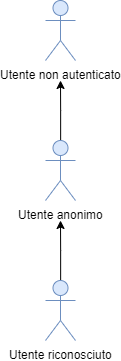
\includegraphics[scale=0.6]{sezioni/UseCase/Immagini/Utenti.png}
\end{figure}

\paragraph{Utente non autenticato}
Utente non ancora autenticato all'applicazione che può avere o non avere le credenziali per autenticarsi.
\paragraph{Utente autenticato}
Utente che si è autenticato e che quindi dispone di credenziali (e-mail e password) per accedere all'applicazione.
\paragraph{Utente anonimo}
Utente autenticato che può venire tracciato all'interno di una organizzazione senza fornire dettagli sulla propria identità.
\paragraph{Utente riconosciuto}
Utente autenticato che può venire tracciato all'interno di una precisa organizzazione fornendo dettagli sulla propria identità.
L'utente si è autenticato presso l'organizzazione tramite LDAP.



\subsubsection{Attori Amministratori}
\begin{figure}[h]
  \caption{Gerarchia degli amministratori}
  \centering
    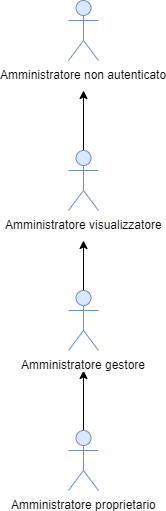
\includegraphics[scale=0.6]{sezioni/UseCase/Immagini/Amministratori.png}
\end{figure}


\paragraph{Amministratore non autenticato}
Amministratore non ancora autenticato nel sistema che ha già le credenziali per autenticarsi.
\paragraph{Amministratore autenticato}
Amministratore che si è autenticato nel sistema.
\paragraph{Amministratore proprietario}
Amministratore autenticatosi con il ruolo di proprietario dell'organizzazione.
Si trova al gradino più alto della gerarchia degli amministratori e dispone delle seguenti funzioni:
\begin{itemize}
\item Gestire l'organizzazione, ovvero modificarne i dati (come nome, descrizione, ecc.) e le superfici geografiche per il tracciamento degli utenti
\item Gestire gli amministratori, cioè la loro nomina, rimozione e modifica dei privilegi
\item Monitorare gli accessi
\item Eliminare l'organizzazione
\end{itemize}
Il proprietario dell'organizzazione può nominare altri amministratori.
\paragraph{Amministratore gestore}
Amministratore autenticatosi con il ruolo di gestore. 
Si trova al secondo gradino della gerarchia degli amministratori e dispone delle seguenti funzioni:
\begin{itemize}
\item Gestire l'organizzazione
\item Monitorare gli accessi
\end{itemize}
\paragraph{Amministratore visualizzatore}
Amministratore autenticatosi con il ruolo di visualizzatore.
Escludendo l'amministratore non autenticato si trova all'ultimo gradino della gerarchia degli amministratori e può compiere solo la seguente funzione:
\begin{itemize}
\item Monitorare gli accessi
\end{itemize}

%Alternativa in caso esista una gerarchia a 3 livelli



